\documentclass[tikz]{standalone}
\usetikzlibrary{calc,patterns,angles,quotes,intersections,positioning,decorations.markings}
\usepackage{pgfplots}
\pgfplotsset{compat=newest}

\pagestyle{empty}
\newcommand{\MarkRightAngle}[4][.2cm]% #1=size (optional), #2-#4 three points: \angle #2#3#4
{\coordinate (tempa) at ($(#3)!#1!(#2)$);
 \coordinate (tempb) at ($(#3)!#1!(#4)$);
 \coordinate (tempc) at ($(tempa)!0.5!(tempb)$);%midpoint
 \draw (tempa) -- ($(#3)!2!(tempc)$) -- (tempb);
}
\begin{document}
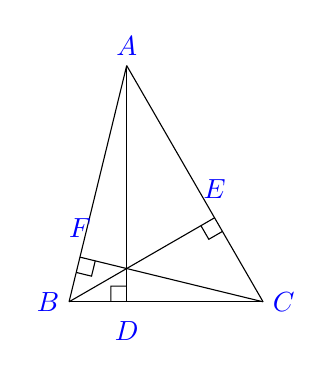
\begin{tikzpicture}

  \coordinate [label={[blue]above:$A$}] (A) at (0, 2);
  \coordinate [label={[blue]right:$C$}] (C) at (1.732, -1);
  \coordinate [label={[blue]left:$B$}] (B) at (-.732, -1);
  \draw (B) -- (C);
  \draw (A) -- (B);
  \draw [name path=AC] (C) -- (A);
  \draw ($(A)!(B)!(C)$) -- (B);
  \draw ($(B)!(A)!(C)$) -- (A);
  \draw ($(B)!(C)!(A)$) -- (C);
  \node [label={[blue]$E$}] () at ($(A)!(B)!(C)$) {};
  \node [label={[blue]below:$D$}] () at ($(B)!(A)!(C)$) {};
  \node [label={[blue]$F$}] () at ($(B)!(C)!(A)$) {};
  \MarkRightAngle {A}{$(B)!(A)!(C)$}{B};
  \MarkRightAngle {B}{$(A)!(B)!(C)$}{C};
  \MarkRightAngle {C}{$(B)!(C)!(A)$}{B};
\end{tikzpicture}
\end{document}
